\usetikzlibrary{matrix, positioning,backgrounds}
\begin{figure}[H]
  \centering
  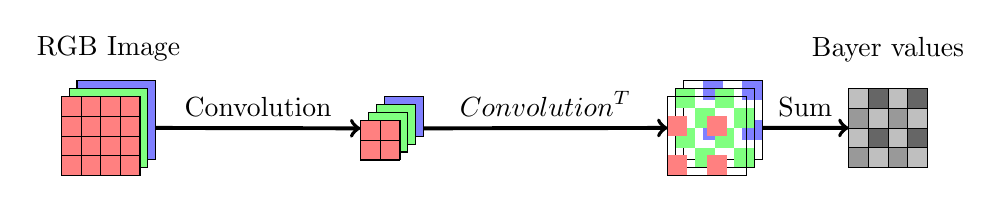
\begin{tikzpicture}
    \begin{scope}[local bounding box=input_layers]
      \filldraw[fill=blue!50]  (0.2,0.2) rectangle (1.2,1.2);
      \filldraw[fill=green!50] (0.1,0.1) rectangle (1.1,1.1);
      \filldraw[fill=red!50]   (0,0)     rectangle (1,1);
      \draw[step=.25,very thin] (0,0) grid (1,1);
    \end{scope}
    \node[] () [above of=input_layers] {RGB Image};
    \begin{scope}[shift={(3.8,0.195)}, local bounding box=inter_layers]
      \filldraw[fill=blue!50]  (0.3,0.3) rectangle (0.8,0.8);
      \filldraw[fill=green!50] (0.2,0.2) rectangle (0.7,0.7);
      \filldraw[fill=green!50] (0.1,0.1) rectangle (0.6,0.6);
      \filldraw[fill=red!50]   (0,0)     rectangle (.5,.5);
      \draw[step=.25,very thin] (0,0) grid (.5,.5);
    \end{scope}
    \begin{scope}[shift={(7.7,0)}, local bounding box=out_layers]
      %\filldraw[fill=green!50]   (0,0)     rectangle (1,1);
      \begin{scope}[shift={(0.2,0.2)}]
      \fill[fill=blue!50] (.25,.25) rectangle (.5,.5);
      \fill[fill=blue!50] (.75,.25) rectangle (1,.5);
      \fill[fill=blue!50] (.25,.75) rectangle (.5,1);
      \fill[fill=blue!50] (.75,.75) rectangle (1,1);
      \draw[very thin] (0,0)     rectangle (1,1);
      \end{scope}
      
      \begin{scope}[shift={(0.1,0.1)}]
      \fill[fill=green!50] (.0,.25) rectangle (.25,.5);
      \fill[fill=green!50] (.5,.25) rectangle (.75,.5);
      \fill[fill=green!50] (.0,.75) rectangle (.25,1);
      \fill[fill=green!50] (.5,.75) rectangle (.75,1);
      \fill[fill=green!50] (.25,.0) rectangle (.5,.25);
      \fill[fill=green!50] (.75,.0) rectangle (1,.25);
      \fill[fill=green!50] (.25,.5) rectangle (.5,.75);
      \fill[fill=green!50] (.75,.5) rectangle (1,.75);
      \draw[very thin]  (0,0)    rectangle (1,1);
      \end{scope}
      
      \fill[fill=red!50]  (0,0)     rectangle (.25,.25);
      \fill[fill=red!50]  (.5,0)    rectangle (.75,.25);
      \fill[fill=red!50]  (.5,.5)   rectangle (.75,.75);
      \fill[fill=red!50]  (0,.5)    rectangle (.25,.75);
      \draw[very thin] (0,0)     rectangle (1,1);
      
    \end{scope}
    \begin{scope}[shift={(10,0.1)}, local bounding box=out_grey]
      \filldraw[fill=black!25]   (0,0)     rectangle (1,1);
      \fill[fill=black!40] (0,0)     rectangle (.25,.25);
      \fill[fill=black!40] (.5,0)    rectangle (.75,.25);
      \fill[fill=black!40] (.5,.5)   rectangle (.75,.75);
      \fill[fill=black!40] (0,.5)    rectangle (.25,.75);
      \fill[fill=black!60] (.25,.25) rectangle (.5,.5);
      \fill[fill=black!60] (.75,.25) rectangle (1,.5);
      \fill[fill=black!60] (.25,.75) rectangle (.5,1);
      \fill[fill=black!60] (.75,.75) rectangle (1,1);
      \draw[step=.25,very thin] (0,0) grid (1,1);
    \end{scope}
    \node[] () [above of=out_grey] {Bayer values};
    \draw[->, line width=.5mm] (input_layers.east) -- node[above] {Convolution} (inter_layers.west);
    \draw[->, line width=.5mm] (inter_layers.east) -- node[above] {$\text{Convolution}^T$} (out_layers.west);
    \draw[->, line width=.5mm] (out_layers.east) -- node[above] {Sum} (out_grey.west);
  \end{tikzpicture}  
  \caption{Synthetic Bayer pipeline}
  \label{fig:rebayer}
\end{figure}
